xo\documentclass[a4paper, 12pt]{article}

\usepackage[english]{babel}
\usepackage[latin1]{inputenc}
\usepackage[T1]{fontenc}

\usepackage{geometry}
\usepackage{fancyhdr}
\usepackage{graphics}

\usepackage{latexsym}
\usepackage{amsmath}
\usepackage{amssymb}

\title{\huge{Graphical Interface for Vaucanson}\\ English abstract}
\author{Guillaume Leroi\\ UID: 18147}

\lhead{Internship's abstract}
\chead{}
\rhead{EPITA 2008}

\geometry{vmargin=3cm, hmargin=3cm}


\begin{document}
\pagestyle{empty}

\maketitle
\thispagestyle{empty}
\newpage

\tableofcontents
\newpage


\pagestyle{fancy}
\setcounter{page}{1}

\section*{Introduction}

Vaucanson is a generic platform dedicated to manipulation and
computation of finite states machines. Generally, automates are
well-known as finite state machine working on letters and answering to
yes-no questions. For example, does a word match a certain regular
expression?
But with Vaucanson, letters can be of any other types (as integers for
example), and the answer is not necessary a boolean value.

Nowadays, Vaucanson interacts with its user by means of a set of
command-line tools, called TAF-KIT.  The purpose of this internship is
to develop a graphical interface for Vaucanson. A prototype already
exists, it has been developed in 2004 by Louis-No�l Pouchet. My work
consists in improving this prototype and its documentation to allow
its distribution.

\begin{figure}[h]
  \centering
  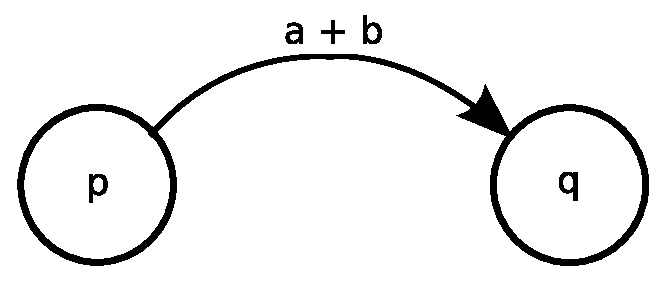
\includegraphics{automaton.eps}
  \caption{Example of an automaton}
\end{figure}

Here is an example of a simple automaton. The terminology is
\begin{itemize}
\item a state: generally draw by a circle.
\item a transition: an arc with a arrow at the end.
\item a label: text above the transition.
\end{itemize}

\section{Internship's context}

ENST is a engineer school based in Paris. Created in 1904, the school
has two main missions: teaching and researching in information
technologies. ENST is also an international school, it receives a lot
of graduate and undergraduate students from all around the world.
ENST's students may also study or follow internship in other countries
through exchange programmes like Erasmus or Mundus.

More precisely, I work in the information technologies and network
department. This department does research on network's flexibility,
distributivity and knowledge management.

My internship supervisor is Jacques Sakarovitch, he is director of
research at CNRS. He is working on the automata theory, teaching it at
ENST for graduate and undergraduate students. Jacques Sakarovitch is
also one of the supervisor of Vaucanson with Akim Demaille (LRDE) and
Sylvain Lombardy (LIAFA).

\subsection{Working conditions}

I have been assigned to a desk, in a room with other students in
different internships. The school lend me a personal computer and an
account.

I have been presented to the administration by my supervisor,
and I meet my self some of the other people of the information
technologies department during my internship, generally near the
coffee machine. People was friendly, and like to speak about their
research and work.

It was very instructive to speak with researchers of this
laboratory, and have an insight on the processing of natural
languages, or network security techniques.



\section{Activity report}

\subsection{Existing materials}

As said before, a prototype of the graphical interface already
exists. The prototype was quite advanced, it allowed to:
\begin{itemize}
\item load and save automata in XML.
\item add and suppress states or transitions.
\item modify the embedding of the automaton.
\end{itemize}
The existing prototype uses the JGraph library. JGraph is a free java
library allowing graph processing and manipulation.

But some problems exist, the prototype was using a old XML format, and
some necessary properties described in the XML file were not used or
misused. Moreover, the code was quite unorganized.

One of the purpose of my internship is to reorganize the code
structure in separate modules, so that future modifications will be
easier. An other purpose is to correctly used properties defined in
the XML format.

\subsection{Accomplished work}

\subsubsection{Reorganization of the code}

The first part of my work has been to read and evaluate the code. I
watch what has been done and where was the problem. I notice that the
code was messy and that not all properties was used.

With the internship's supervisor, a software design has been decided.
Four modules have been described, each representing a set of
functionalities:
\begin{itemize}
\item XML module: save and load automata to our XML format.
\item Geometry module: set and get geometry properties of an
  automaton, define default values and manipulation methods.
\item Drawing module: same as geometry module, but for drawing
  properties.
\item Translation module: translate geometry and drawing properties,
  type information to JGraph.
\end{itemize}

\paragraph{XML module:}

The XML module already exists in the first prototype, but it was using
an old XML format. So, the module has been updated with respect to the
newer XML format. Properties are now correctly saved to XML
attributes, using good units.

\paragraph{Geometry module:}

Geometry properties give informations on the automaton embedding. For
example:
\begin{itemize}
\item coordinates of a state.
\item informations on the shape of a transition: is it a arc? or a line?
\item where the label of a transition is on its transition?
\end{itemize}

The geometry module gives methods to manipulate the map of geometry
properties.
\begin{itemize}
\item when setting a value, the module checks if the value is correct.
\item if no value has been defined is the XML file, the module put
  forward a default value.
\item the module defines too some utility functions, coordinates
  conversion from the fictive coordinates of XML to screen
  coordinates.
\end{itemize}

The geometry module defines too some layouts. A layout defines the
``shape'' of an automaton. The prototype already defines some
layouts, allowing the user to arrange states in circle, square and
other shapes. So they have been moved to the geometry module, and
modified to use the functionalities and informations provide by the
geometry properties.

\paragraph{Drawing module:}

Drawing properties give informations on how to draw an automaton. For
example:
\begin{itemize}
\item the color of a state.
\item the thickness of a transition.
\item the distance between a label and its transition.
\end{itemize}

The drawing module globally offers the same functionalities than the
geometry module, but for drawing properties. The drawing module puts
forward methods to get and set values of drawing properties, checking
if the given value is correct.

\paragraph{Translation module}

Preceding modules use and modify internal values, but the prototype
use a special library called JGraph to draw the automaton. So this
internal properties need to be expose to JGraph.

By reading already existing codes and JGraph documentation, the
translation module has been populated by different classes, each class
translating a limited set of properties.

\begin{itemize}
\item Router class: translate the transition type. It explains to
  JGraph how to draw an arc, or a line.
\item StateView class: this class explains to JGraph how to draw a state.
\item TransitionView class: use geometry and drawing properties to
  explain to JGraph how and where to draw the label of a transition.
\end{itemize}

\subsubsection{Documentation}

To allow its distribution and future enhancements, the graphical
interface needs documentations. A user manual already exists, but
nothing for developers. So a developer documentation is in progress,
it describes the code structure. It describes too each module, with
its purpose, its classes and where particular computations are done.
Therefore, future enhancements and bug corrections will be make
easier.

\subsection{Acquired skills}

The execution of this project gives the occasion to learn some new
skills. The prototype is written in Java, so it was the occasion to
discover this language and its libraries.

I had the opportunity to use and discover capacities of the
following libraries:
\begin{itemize}
\item JGraph: a graph component library.
\item Swing: a user interface components library, widely used by other
  projects all around the world.
\item DOM parser: it is the java API to parse XML documents, and
  manipulate them. XML is more and more used, becoming a standard
  format for exchanging informations.
\item and all the standard java libraries.
\end{itemize}

I had also the opportunity to discover Eclipse, a integrated
development environment. This software has great capabilities for
debugging and refactoring java programs.



\section{Conclusion}

Even if the result of my work is still a prototype, it is quite
usable. The new design and documentations will make easier future
modifications. Developing a java-based application was quite
interesting, it makes me discover the strength and weakness of Java
and give me a little overview of what can be done with this framework.
Moreover, using Java gives us portability, which important for this
project. The application was developed on Unix, but my supervisor runs
it on Mac. No modifications were needed.

Some critics could be express about the project, mainly on the choice
of Java and JGraph. Even if there are great technologies with a lot of
features, they don't feet all our needs. Java is sometime a too
low-level language for what we want to do, and JGraph does not offer a
way to display objects which is not based on pixel.

Maybe, for the next prototype, we should look towards over displaying
technologies, like vector based graphics.



\end{document}
